\documentclass{article}
\usepackage{titling}
\usepackage{lipsum}
\usepackage{amsmath}
\usepackage{listings}
\usepackage{graphicx}
\usepackage{subcaption}
\usepackage{pgfplots}
\usepgfplotslibrary{statistics}



\begin{document}
\noindent
\begin{minipage}[t]{0.6\textwidth}
    \begin{flushleft}
        \LARGE\textbf{Math 343 - Homework 2} \\
        \vspace{6pt} % add 6pt of vertical space
        \hrule width 10cm
        \vspace{12pt}
        \large\textbf{Preston Duffield} \\
        \large Western Washington University \\
        % \today
        April 14, 2023
        \vspace{24pt}
    \end{flushleft}
\end{minipage}

\section*{Question 1}

Data with a rightward skew would produce a normal probability plot with a positive curvature.
Below is an example of a histogram that would produce a positively curved normal probability plot. \\


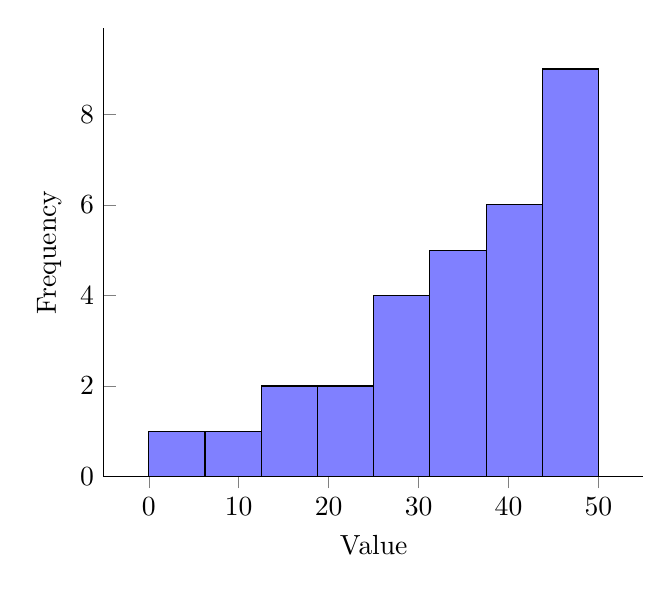
\begin{tikzpicture}
  \begin{axis}[
      ybar,
      ylabel={Frequency},
      xlabel={Value},
      ymin=0,
      axis lines*=left,
      % xtick=data,
      % nodes near coords,
      % nodes near coords align={vertical},
  ]
  \addplot[
      fill=blue!50,
      hist={
          bins=8,
          data min=0,
          data max=50,
      },
  ] table[row sep=\\,y index=0] {
      data \\
      36 \\ 30 \\ 25 \\ 40 \\ 50 \\ 6 \\
      35 \\ 9 \\ 50 \\ 24 \\ 40 \\
      15 \\ 16 \\ 50 \\ 50 \\ 21 \\
      25 \\ 50 \\ 40 \\ 30 \\ 32 \\
      35 \\ 36 \\ 38 \\ 40 \\ 42 \\
      45 \\ 46 \\ 48 \\ 50 \\
  };
  \end{axis}
  \end{tikzpicture}
\clearpage
\section*{Question 2}

$H_0$: $\mu_1 - \mu_2 = 10$ \\
$H_a$: $\mu_1 - \mu_2 > 10$ \\

\begin{align*}
  Z &= \frac{\bar{y}_1 - \bar{y}_2 - 10}{\sqrt{\frac{\sigma_1^2}{n_1} + \frac{\sigma_2^2}{n_2}}} \\
    &= \frac{162.5 - 155 - 10}{\sqrt{\frac{1^2}{10} + \frac{1^2}{12}}} \\
    &= -5.838
\end{align*}

By observing that $Z_{\alpha} = 3.09$ we can conclude the following.
There is not enough statistical evidence to support the hypothesis that $\mu_1 - \mu_2 = 10$,
ie, the breaking strength of plastic 1 exceeds that of plastic 2 by at least 10 psi.
Therefore, based on the sample information, they should not use plastic 1. \\

A $100(1-\alpha)$ confidence interval is given by:
\begin{align*}
  100(1-\alpha) \text{ C.I} = \bar{y}_1 - \bar{y}_2&\pm Z_{\alpha/2} \sqrt{\frac{\sigma_1^2}{n_1} + \frac{\sigma_2^2}{n_2}} \\
  7.5                       &\pm 3.29 \sqrt{\frac{1^2}{10} + \frac{1^2}{12}} \\
  7.5                       &\pm 1.40
\end{align*}

We are 99\% confident that the true value of $\mu_1 - \mu_2$ is between 6.1 and 8.9.
This is consistent with our above test which conlucded that the difference was not greater than 10.
\clearpage
\section*{Question 3}

\subsection*{a)}
\begin{figure}[h]
    \centering
    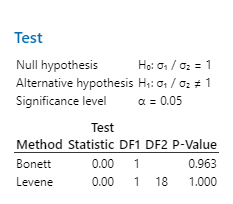
\includegraphics[width=0.5\textwidth]{./images/3_a.png}
    \caption{The output of the test for two variances from Minitab.}
    \label{fig:3_a}
  \end{figure}
  Since the P-value $> \alpha$ we can conclude the following.
  There is enough statistical evidence to support the hypothesis that both of the variances are equal.

\subsection*{b)}
\begin{figure}[h]
    \centering
    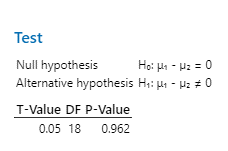
\includegraphics[width=0.5\textwidth]{./images/3_b.png}
    \caption{The output of the two sample t test from Minitab. Assuming equal variances.}
    \label{fig:3_a}
  \end{figure}
  Since the P-value $= 0.962 > \alpha$ we can conclude the following.
  There is enough statistical evidence to support the hypothesis that the two means are equal.

  \clearpage
  \subsection*{c)}

\begin{figure}[h]
    \centering
    \begin{subfigure}[b]{0.4\textwidth}
        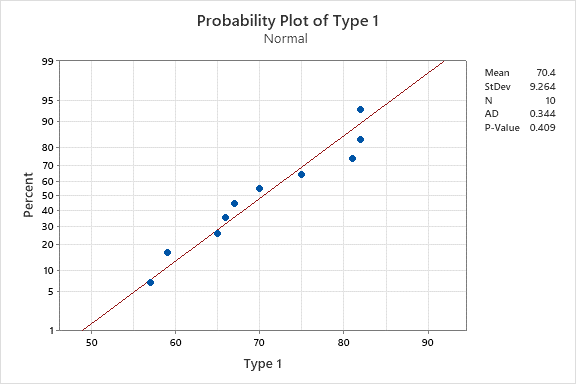
\includegraphics[width=1.25\textwidth]{./images/3_c_1.png}
        \caption{Minitab output showing the probability plot of type 1.}
      \label{fig:img1}
    \end{subfigure}
    \hfill
    \begin{subfigure}[b]{0.4\textwidth}
        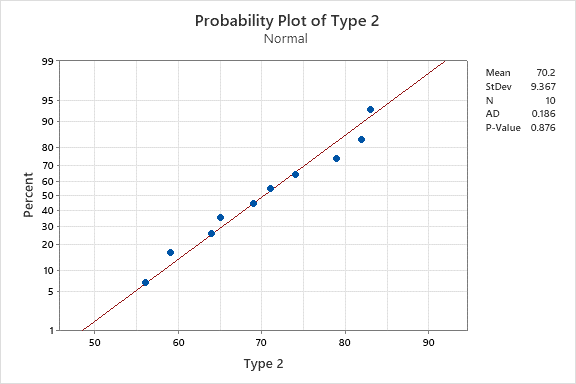
\includegraphics[width=1.25\textwidth]{./images/3_c_2.png}
        \caption{Minitab output showing the probability plot of type 2.}
      \label{fig:img2}
    \end{subfigure}
    \label{fig:both}
  \end{figure}

  Note that for both Type 1 and Type 2, the hypothesis we will test is as follows. \\
  $H_0$: The data are drawn from a normal distribution. \\
  $H_a$: The data are not drawn from a normal distribution. 

\paragraph{Type 1} Since the P-value $= 0.409 > \alpha$ we can conclude the following.
    The evidence of the data is consistent with the hypothesis that the data are drawn from a normal distribution.

\paragraph{Type 2} Similarly, since the P-value $= 0.876 > \alpha$ we can conclude the following.
    The evidence of the data is consistent with the hypothesis that the data are drawn from a normal distribution.

\clearpage
\section*{Question 4}
\subsection*{a)}
The hypothesis to test whether insulation has reduced the average energy consumption is: \\
$H_0$: $\delta = 0$ \\
$H_a$: $\delta > 0$ \\
This will be a right-tailed paired t-test at $\alpha = 0.1$.
\begin{equation*}
  \begin{array}{c|c}
      \text{Sample Mean of differences} & \bar{d} = 0.54 \\
      \text{Sample Standard Deviation of differences} & S_d = 1.01566\\
      \text{Sample Size} & n = 10 \\
  \end{array}
\end{equation*}\\
The test statistic $t$ is:
\begin{align*}
  t = & \frac{\bar{d}}{S_d/\sqrt{n}} \\
    = & \frac{0.54}{1.01566/\sqrt{10}} \\
    = & 1.681 \\
\end{align*}
The critical region begins at:
\begin{equation*}
t_{\alpha , n-1} = t_{.1,9} = 1.383
\end{equation*}\\

Since $t = 1.681 > t_{.1,9} = 1.383$,
that is, the test statistic is in the right-tailed critical region we can conclude the following.
There is enough statistical evidence to support the hypothesis that $\delta > 0$, ie,
the mean energy consumption after insulation is less than the mean eneergy consumption before insulation.

\subsection*{b)}

\paragraph{1.} One factor that could have affected the results is the mean difference in temperature between the two winters.
If one winter was significantly colder than another it could have affected the data that was collected.

\paragraph{2.} Another factor that could have affected the result is that other electronic appliances could have significantly affected the energy consumption.
If there was a significant difference in the energy consumption of other appliances between the two winters it could have affected the results.

\clearpage
\section*{Question 5}

\subsection*{a/b)}

\begin{figure}[h]
  \centering
  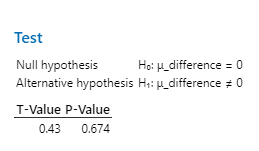
\includegraphics[width=0.5\textwidth]{./images/5_a_1.png}
  \caption{The output of the paired t test from Minitab.}
  \label{fig:5_a}
\end{figure}
Since the P-value $= 0.674 > \alpha$ we can conclude the following.
There is enough statistical evidence to support the hypothesis that the two means are equal.

\subsection*{c)}

\begin{figure}[h]
  \centering
  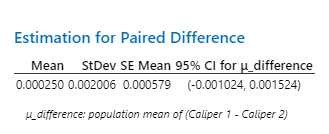
\includegraphics[width=0.5\textwidth]{./images/5_a.png}
  \caption{The output of the paired t test containing the confidence interval from Minitab.}
  \label{fig:5_a}
\end{figure}
From the above confidence interval we can conclude the following.
We are 95\% confident that the true difference between the population means is between -0.001 and 0.001.

We can also note that the confidence interval contains 0, which is consistent with our hypothesis test.

\clearpage
\section*{Question 6}

\subsection*{a)}
\begin{lstlisting}[language=R, caption=R output of Shapiro-Wilk test on Birth Order: 1, basicstyle=\small]
                Shapiro-Wilk normality test

                data:  b1
                W = 0.84597, p-value = 0.05201
\end{lstlisting}

Since the P-value $= 0.05201 > \alpha$ we can conclude the following.
    The evidence of the data is consistent with the hypothesis that the data are drawn from a normal distribution.



\begin{lstlisting}[language=R, caption=R output of Shapiro-Wilk test on Birth Order: 1, basicstyle=\small]
                Shapiro-Wilk normality test

                data:  b2
                W = 0.92972, p-value = 0.4452
\end{lstlisting}

Since the P-value $= 0.4452 > \alpha$ we can conclude the following.
    The evidence of the data is consistent with the hypothesis that the data are drawn from a normal distribution.


\subsection*{b)}

\begin{lstlisting}[language=R, caption=R output of a paired t test, basicstyle=\small]
                Paired t-test

                data:  b1 and b2
                t = -0.36577, df = 9, p-value = 0.723
                alternative hypothesis:
                    true mean difference is not equal to 0
                95 percent confidence interval:
                    -0.3664148  0.2644148
                sample estimates:
                mean difference 
                    -0.051 
\end{lstlisting}

The confidence intercal on the difference in mean score leads us to the following conclusion.
We are 95\% confident that the true difference in the population means is between -0.36 and 0.26.
Since the confidence interval contains 0, we can also conclude that the two sample means may be equal.

\subsection*{c)}

\begin{flushleft}
  $H_0$: $\mu_1 = \mu_2$ \\
  $H_a$: $\mu_1 \neq \mu_2$ \\
\end{flushleft}

Since the P-value $= 0.723 > \alpha$ we can conclude the following.
There is enough statistical evidence to support the hypothesis that the sample means are equal,
ie, $\mu_1 = \mu_2$.


\section*{Question 7}

To test the hypothesis that the true
population variance of Formulation 1 (new recipe),
is greater than the true population variance of Formulation 2 (original recipe)
, we will use the following hypothesis: \\
$H_0$: $\sigma_1^2 = \sigma_2^2$ \\
$H_a$: $\sigma_1^2 > \sigma_2^2$ \\

This will be a right tailed test of two variances at $\alpha = 0.05$.
The test statistic for the test is:
\begin{align*}
  F = & \frac{S_1^2}{S_2^2} \\
    = & \frac{0.100}{0.061} \\
    = & 1.639 \\
\end{align*}
The critical region begins at:
\begin{equation*}
F_{\alpha , n_2-1, n_1-1},  = F_{.05 , 9, 9} = 3.18
\end{equation*}\\

Since $ F = 1.639 <  F_{.05 , 9, 9} = 3.18$, the test statistic is not in the right-tailed critical region
we can conclude the following.
There is enough statistical evidence to support the hypothesis that $\sigma_1^2 > \sigma_2^2$, ie,
the true
population variance of Formulation 1 (new recipe),
is greater than the true population variance of Formulation 2 (original recipe).

\clearpage
\section*{Question 8}
To derive the confidence interval for the ratio $\frac{\sigma_1^2}{\sigma_2^2}$ we can start with the fact that
$\frac{S_1^2 / \sigma_1^2}{S_2^2 / \sigma_2^2}$
has an $F$ distribution with $n_1 - 1$ numerator
degrees of freedom and $n_2 - 1$ denominator degrees of freedom. This insight leads to:
\begin{align*}
1 - \alpha  & = P\left( F_{1 - \frac{\alpha}{2}, n_1 - 1, n_2 - 1} < \frac{S_1^2 / \sigma_1^2}{S_2^2 / \sigma_2^2} < F_{\frac{\alpha}{2}, n_1 - 1, n_2 - 1} \right) \\
            & = P\left( F_{1 - \frac{\alpha}{2}, n_1 - 1, n_2 - 1} \cdot \frac{S_2^2}{\sigma_2^2} < \frac{S_1^2}{\sigma_1^2} < F_{\frac{\alpha}{2}, n_1 - 1, n_2 - 1} \cdot \frac{S_2^2}{\sigma_2^2} \right) \\
            & = P\left( \frac{S_1^2}{S_2^2} < \frac{\sigma_1^2}{\sigma_2^2} < \frac{F_{\frac{\alpha}{2}, n_1 - 1, n_2 - 1}}{F_{1 - \frac{\alpha}{2}, n_1 - 1, n_2 - 1}} \cdot \frac{S_1^2}{S_2^2} \right) \\
\end{align*}
Therefore the $100(1-\alpha)$ confidence interval for the ratio of variances is given by:
\begin{equation*}
  \frac{\sigma_1^2}{\sigma_2^2} \in \left( \frac{S_1^2}{S_2^2} \cdot \frac{1}{F_{\frac{\alpha}{2}, n_1 - 1, n_2 - 1}}, \frac{S_1^2}{S_2^2} \cdot \frac{1}{F_{1 - \frac{\alpha}{2}, n_1 - 1, n_2 - 1}} \right)
  \end{equation*}\\
\end{document}
